\chapter[Concetti preliminari]{Concetti preliminari}\label{chap:preliminaries}
Per poter considerare l'utilizzo dei tipi per il Web Semantico, è necessario analizzare lo stato dell'arte in cui si ritrova questo ambito di ricerca.
Questo capitolo si presta utile per apprendere il vocabolario utilizzato durante tutta la tesi, nonché fornire approfondimenti su nozioni che potrebbero essere date per scontate.
Verranno riassunte le basi dei linguaggi funzionali, così come le componenti del Web Semantico.
\section[Linguaggi funzionali]{Linguaggi funzionali}

\section[Web Semantico]{Web Semantico}
Il World Wide Web è diventato una consolidata rete di conoscenza, che però presenta il difetto che queste informazioni sono pensate per la fruizione umana, piuttosto che da parte di una macchina. Infatti il linguaggio di rappresentazione delle centinaia di pagine che visitiamo ogni giorno, l’HTML, descrive l’impaginazione delle informazioni visualizzate all’utente. Senza un indicazione che spiega il significato dei dati presenti, un agente intelligente non può interpretarne il significato. Uno degli obiettivi del Web Semantico, termine che risale all'articolo del 2001 di Tim-Berners Lee \cite{berners2001semantic}, è cambiare questo paradigma human-centered, permettendo agli agenti artificiali di interpretare e processare la conoscenza presente senza alcun tipo di aiuto umano. È necessario descrivere le informazioni attraverso metadati espressivi, strutturandoli arbitrariamente, che ne spieghino la semantica in un modo che una macchina possa comprenderla.\\
Nel corso degli anni, nella letteratura sono state presentate diverse soluzioni: dagli albori di questo ambito, in cui i dati erano rappresentati in maniera strutturata e formale dalle ontologie, si è giunti alla rappresentazione superficiale ma efficiente del paradigma dei Linked (Open) Data. Questa sezione vuole introdurre agli standard di rappresentazione e recupero dei dati citati in questo lavoro.



\subsection[Resource Description Framework]{Resource Description Framework}
Il Resource Description Framework \cite{RDFspecification} (RDF d'ora in poi) è una serie di specifiche create da W3C (World Wide Web Consortium) che includono un modello per descrivere risorse web attraverso delle annotazioni, sotto forma di \textbf{triple}. Esse consistono in:
\[ < \text{soggetto},\ \text{predicato},\ \text{oggetto} > \]
Un insieme di queste triple, chiamato \textbf{grafo RDF}, può essere rappresentato come un grafo diretto etichettato in cui ogni tripla descrive un arco dal nodo soggetto al nodo oggetto.
\begin{figure}[h]
    \begin{minipage}{0.3\linewidth}
        \centering
        \begin{tikzpicture}[
                node distance = 15mm and 15mm,
                V/.style = {rounded corners, draw, fill=gray!30},
                every edge quotes/.style = {auto, font=\footnotesize, sloped}
            ]
            \begin{scope}[nodes=V]
                \node (1)   {Pizza};
                \node (2) [right=of 1]    {Margherita};
                \node (3) [below =of 2]    {Mozzarella};
                \node (4) [left=of 3]    {Vegetarian};
            \end{scope}
            \draw[->, ultra thick]   (2)  edge["isA"] (1)
            (2)  edge["madeOf"] (3)
            (4)  edge["canEat"] (2);
        \end{tikzpicture}
    \end{minipage}
    \hspace{5mm}
    \begin{minipage}{0.7\linewidth}
        \begin{alignat*}{4}
            G_1 = \{ (\  & \text{Margherita},\  &  & isA,      &  & \text{Pizza}        &  & ),  \\
            (\           & \text{Margherita},\  &  & madeOf,\  &  & \text{Mozzarella}\  &  & ),  \\
            (\           & \text{Vegetarian},\  &  & canEat,\  &  & \text{Mozzarella}\  &  & )\}
        \end{alignat*}
    \end{minipage}
    \caption{un grafo RDF $G_1$ come grafo diretto (sx.) e insieme di triple (dx.)}
    \label{fig:grafoRDF}
\end{figure}

\noindent
Per essere più precisi, \textit{in RDF sia i nodi che i predicati sono risorse}, cioè delle entità nell'universo del discorso d'interesse. A seconda che la risorsa sia una stringa (come Margherita nella \autoref{fig:grafoRDF}) oppure un concetto più astratto è possibile identificarla in due modi diversi: tramite IRI oppure come un letterale. In ogni caso, definire una tripla RDF significa dire che la relazione indicata dal predicato vale fra le risorse indicate dal soggetto e dall'oggetto. Parliamo meglio di questi metodi d'identificazione:
\begin{description}
	\item[IRI (International Resource Identifier)]  Un formato generalizzato di URI che ricorre a un range più ampio di caratteri Unicode, che permette di identificare univocamente una risorsa. È importante sapere che solamente gli IRI vengono utilizzati per identificare i predicati in una tripla, e denotano una \textbf{proprietà}, cioè una risorsa che può essere vista come una relazione binaria.
	Un insieme di IRI destinati all'uso in un grafo RDF è chiamato \textbf{vocabolario RDF} e di solito tutti gli identificatori di uno stesso vocabolario condividono una sotto stringa iniziale comune, che prende il nome di \textbf{namespace}. Per migliorare la leggibilità dei documenti RDF, si utilizza un \textbf{prefisso}, che sostituisce il namespace per abbreviare la lunghezza del identificatore. Ad esempio, per l'IRI \verb|http://example.org/#Margherita| si potrebbe definire il namespace\\ \verb|http://example.org/#| con prefisso \verb|example|; in questo modo la risorsa Margherita può essere identificata con il più corto e leggibile \verb|example:Margherita|. Alcuni esempi concreti possono esseri trovati in \cite{RDFSspecification}.
	\item[Letterali] Rappresentano risorse nel senso di valori numerici, date o stringhe. La codifica di un qualsiasi valore di un letterale è come stringa Unicode, ma è possibile specificare il tipo, identificato da un IRI (e.g. il tipo delle date è \verb|xsd:date|), per permettere di risalire alla vera semantica del valore.
\end{description}
Esiste anche un altro termine che permette di affermare la presenza di un nodo per cui sussiste la relazione, senza nominarlo in maniera esplicita: il \textbf{blank node}. Per fare un paragone, possono essere considerati come variabili esistenziale, in cui il valore non è conosciuto ma si assume che sia presente.

\begin{definition}[Tripla RDF]
	Siano \textbf{I}, \textbf{L} e \textbf{B} rispettivamente gli insiemi infiniti e disgiunti uno a uno delle stringhe IRI, dei letterali e dei blank nodes. Una tripla RDF è una tupla $(s, p, o) \in \textbf{U}\ \cup \textbf{B} \times \textbf{U} \times \textbf{U}\ \cup \textbf{B}\ \cup \textbf{L}.$ in cui s è chiamato soggetto, p il predicato e o l'oggetto.
\end{definition}
\begin{definition}[Grafo RDF]
	Un grafo RDF è un insieme finito di triple RDF.
\end{definition}
\begin{definition}[Grafo RDF]
	Un grafo RDF è un insieme finito di triple RDF.
\end{definition}
IRI (International Resource Identifier),

\subsection{SPARQL CQ}
I grafi RDF vengono interrogati utilizzando le query SPARQL, infatti i grafi vengono memorizzati in database speciali chiamati triplestore, per efficentare le interrogazioni. In questa trattazione utilizziamo un tipo particolare di SPARQL, le query congiuntive, che consistono nella congiunzione di triple pattern, elementi atomici per interrogare un triplestore. \\
\textbf{Abitabilità: } In una query SPARQL, il concetto di abitabilità identifica le query che possono essere abitate da almeno un elemento. Per esempio, se scriviamo una query che richiede tutti i nodi che sono sia di classe Pizza sia di classe Gelato, ovviamente questa query non potrà mai essere abitata, perchè non esistono pizze che allo stesso tempo sono anche dei gelati. Il concetto di abitabilità però non è da confondere con il fatto che essa sia abitata: una query potrebbe essere abitata, ma nel grafo RDF su cui stiamo lavorando non c'è nessun nodo che soddisfa i requisiti. \ 
\begin{figure}[H]
    \centering
    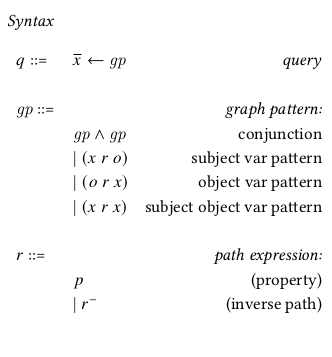
\includegraphics[scale=0.6]{pictures/leinbergSyntax}
    \caption{sintassi delle query \\ SPARQL CQ}
    \label{fig:leinbergerSyntax}
\end{figure}
\newpage
\section[Ontologie]{Ontologie}
La definizione comunemente accettata di ontologia è \textit{una specifica formale ed esplicita di una concettualizzazione condivisa} \cite{goy2015ontologies}. Un modo di rappresentarle è attraverso particolari linguaggi altamente espressivi appartenenti a una famiglia di formalismi chiamati logiche descrittive (DL). Le informazioni sul dominio di interesse vengono espresse in maniera formale tramite formule logiche di due tipologie. Una tipologia fa parte della cosiddetta T-Box e sono asserzioni sulla terminologia, componendo uno schema. L'altra fa parte della A-Box ed è usata per fare asserzioni su individui (astratti), quindi modella le istanze significative. Il T-Box contiene formule logiche (assiomi) che mettono in relazione delle \textit{concept expressions} per modellare il dominio di riferimento, ad esempio il fatto che  uno Student è una Persona. Una \textit{base di conoscenza} è quindi l'insieme di asserzioni presenti sia nel T-Box che nell'A-Box.\\
Nel contesto del Web Semantico, la raccomandazione W3C \textit{Web Ontology Language (OWL)} è una famiglia di linguaggi ontologici altamente espressivi basati sul linguaggio descrittivo $\mathcal{SROIQ}$ \cite{baader2017introductionDL}. Quello che andremo a mostrare noi nella sezione dei costrutti sintattici DL è il più semplice sottoinsieme $\mathcal{ALCOIQ}$.
Grazie alla forma logica delle informazioni, è possibile definire un ragionamento automatico\footnote{\ i.e. tramite un algoritmo deterministico, cioè eseguibile da un computer} che permette di svolgere operazioni di inferenza sugli individui concreti, ad esempio inferire che il nodo \textit{x} di un grafo RDF è uno Studente, ma anche eseguire compiti più astratti, come capire se un concetto è soddisfacibile. Questi compiti sono alla base di ogni reasoner, come ad esempio HermiT \cite{HermiT}, Pellet \cite{Pellet} e Fact++ \cite{Fact++}.\\

\subsection[Logica  descrittiva $\mathcal{ALCOIQ}$]{Logica  descrittiva $\mathcal{ALCOIQ}$}
Questa introduzione e gli esempi sono presi dal libro \cite{baader2017introductionDL}, che contiene un'ottima introduzione alle logiche descrittive. Per non divagare troppo dal motivo per cui spieghiamo questi concetti, ovvero per permettere ai lettori meno esperti delle ontologie di capire la terminologia usata in questa tesi, la logica utilizzata in questa sezione sarà principalmente $\mathcal{ALCOIQ}$. Per questo motivo, useremo anche esempi e tabelle prese dall'introduzione della tesi di dottorato di Leinberger \cite{leinbergerphdthesis}. L'acronimo $\mathcal{ALCOIQ}$ descrive i costrutti sintattici disponibili nel linguaggio (\autoref{fig:SintassiCD}). I costrutti di base sono contenuti in $\mathcal{ALC}$ (\textit{Attributive Language with Complements}), e le estensioni introdotte sono spiegate nella \autoref{tab:ALCOIQExtensions}. \\\\
I linguaggi appartenenti alle logiche descrittive separano le informazioni di un argomento in una parte terminologica (\textit{T-Box}) e una di asserzioni (\textit{A-Box})\footnote{ Nelle estensioni $\mathcal{R}$ del linguaggio $\mathcal{ALC}$, come ad esempio in OWL ($\mathcal{SROIQ}$), esiste una terzo insieme di asserzioni chiamati R-Box. Dentro vengono contenute asserzioni per creare legami fra i ruoli (come equivalenza o sotto-ruolo). Per saperne di più consultare \cite{baader2017introductionDL}}. In altre parole, il T-Box definisce informazioni sulla correlazioni dei concetti (e.g. Studente è una Persona che frequenta un corso), simile a uno schema di un database. L’A-Box descrive invece la rappresentazione concreta dei concetti (e.g. Alice è una Persona), molto più simile alle istanze di una tabella relazionale. La combinazione di entrambe viene definita una \textit{Knowledge Base} (KB).
Nelle logiche descrittive si assume di voler descrivere un’astrazione della realtà d’interesse, e che questa sia popolata da elementi. Per descrivere quest'ultimi utilizziamo tre componenti:
\begin{description}
	\item[Concept expression] Anche chiamato concept description, è un insieme di elementi e può essere visto come un predicato unario. Le concept expressions sono definite a partire dai \textit{nomi di concetti} e dai \textit{nomi di ruolo}. Sono definiti induttivamente dall’insieme di tutte le regole sintattiche del linguaggio considerato (vedi \autoref{fig:SintassiCD}). L’insieme che una concept description rappresenta è chiamato la sua \textit{estensione}. Per esempio, Persona è un concetto, e Alice è un elemento (nell’estensione) di Persona.
	\item[Role expression] relazione binaria sugli elementi. È definito atomicamente da un \textit{nome}. L'unico altro costrutto in $\mathcal{ALCOIQ}$ è il ruolo inverso, che non è nient'altro che la coppia di entità in ordine inverso. Se un ruolo \textit{r} mette in relazione un elemento con un altro, si definisce quest’ultimo un \textit{r}-filler del primo (es. Alice \textit{insegna} C, C è un \textit{insegna}-filler di Alice).
	\item[Linguaggio concettuale] il linguaggio formale al centro di uno specifica logica descrittiva. Permette di costruire concept expressions e role descriptions partendo da nomi di concetti, nomi di ruoli e altre primitive.
\end{description}

Di solito un linguaggio DL permette di costruire concetti utilizzando gli operatori comuni alla logica del prim’ordine (e.g. $\sqcap, \sqcup, \exists, \forall \text{ e } \neg)$, ma ci possono essere varie estensioni che possono essere considerate per un linguaggio. L'estensione che può risultare più strana nella \autoref{fig:SintassiCD} è la regola (Restrizione num. richiesto), che richiede che permette di esprimere il vincolo di avere almeno \textit{n} \textit{r}-filler della concept expression C. Per fare un esempio servirebbe definire l'ambito in cui vengono utilizzate le concept e le role expression, che è proprio quello che introdurremo nella sezione successiva.\\
\begin{figure}[b!]
	\begin{center}	
		\begin{minipage}{0.6\textwidth}
			\setlength{\grammarindent}{3em} % increase separation between LHS/RHS 
			\begin{grammar}
				\let\syntleft\relax
				\let\syntright\relax
				<$\mathbf{C}$> ::= $c$ \hfill (Concetto atomico)
				\alt $\{o\}$ \hfill (Concetto nominale)
				\alt $\top$ \hfill (Top)
				\alt $\bot$ \hfill (Bottom)
				\alt $\neg \mathbf{C} $ \hfill (Negazione)
				\alt $\mathbf{C} \sqcap \mathbf{C}$ \hfill (Congiunzione)
				\alt $\mathbf{C} \sqcup \mathbf{C}$ \hfill (Disgiunzione)
				\alt $\exists\ \mathbf{R}. \mathbf{C}$ \hfill (Esistenziale)
				\alt $\forall\ \mathbf{R}. \mathbf{C}$ \hfill (Universale)
				\alt $\ge n\ \mathbf{R} . \mathbf{C}$ \hfill (Restrizione num. richiesto)
				
				<$\mathbf{R}$> ::= $r$ \hfill (Ruolo atomico)
				\alt $\mathbf{R}^-$ \hfill (Ruolo inverso)
			\end{grammar}
		\end{minipage}
		\caption{sintassi delle \textit{concept expressions} $\mathbf{C}$ e delle \textit{role descriptions} $\mathbf{R}$}
		\label{fig:SintassiCD}
	\end{center}
\end{figure}

\begin{table}
	\centering
	\begin{tabular}{c l c}
		\hline
		Estensione & Descrizione & Costrutto \\
		\hline
		$\mathcal{O}$ & Concetti nominali & $\{o\}$\\
		$\mathcal{I}$ & Ruoli inversi & $ \mathbf{R} ^-$\\
		$\mathcal{Q}$ & Restrizione del numero richiesto & $\ge n\ \mathbf{R} . \mathbf{C} $\\
		
		\hline
	\end{tabular}
	\caption{estensioni dei costrutti sintattici nel DL $\mathcal{ALCOIQ}$}
	\label{tab:ALCOIQExtensions}
\end{table}
In questa introduzione vedremo in particolare il linguaggio concettuale su cui si basa una semplificazione di OWL per permettere ai lettori meno esperti di comprendere il codice presente nel \autoref{chap:Implementazione}.
\noindent
Vedremo a breve il significato della semantica di questi costrutti, ma vale la pena di spendere qualche parola su come andranno a essere utilizzati alcuni di essi. In particolare, esistono diversi costrutti per andare a specificare degli insiemi per tutti quegli elementi che sono in relazione con un certo ruolo a un concetto particolare (parliamo di $\exists r. \mathbf{C}$,  $\forall r. \mathbf{C}$ e $\ge n\ \mathbf{R} . \mathbf{C}$). Questo ci permetterà principalmente nel T-Box di dichiarare qualche genere di concetto che deve essere in relazione con qualcosa. Ad esempio, un Celibe è un uomo che non ha consorte, ed è proprio la mancanza a caratterizzare gli elementi nell'estensione di Celibe. Questo si potrebbe andare a caratterizzare con la concept expression $\text{Uomo}\sqcap \neg\ \exists\ \textit{spostatoCon}. \text{Consorte}$.\\
Una cosa da notare è che la regola (Esistenziale) potrebbe essere espressa attraverso la (Restrizione num. richiesto). Infatti, $\exists r. \mathbf{C}$ è intuitivamente equivalente al caso particolare $\ge 1\ \mathbf{R}. \mathbf{C}$. Per un elenco di regole derivate consultare la sezione 2.2.3 di \cite{leinbergerphdthesis}.


\subsubsection*{Semantica DL}
La semantica nelle logiche descrittive è intesa attraverso un'interpretazione $\mathcal{I}$, definita come segue.
\begin{definition}
	Un'interpretazione $\mathcal{I}$ è una struttura del tipo $\mathcal{I} = (\triangle^\mathcal{I}, \cdot^\mathcal{I})$, dove $\triangle^\mathcal{I}$ è un insieme non vuoto chiamato \textit{dominio d’interpretazione} e $\cdot^\mathcal{I}$ è la \textit{funzione di interpretazione} che mappa ogni costrutto alla sua semantica definita nella \autoref{tab:SintaxSemanticsALCOIQ}.
\end{definition}
\noindent
Come è possibile intuire dalla \autoref{tab:SintaxSemanticsALCOIQ}, ai costrutti della logica descrittiva (concetti e ruoli) vengono assegnati dei significati insiemistici.
\begin{table}[t!]
	\centering
	\footnotesize
	\begin{tabular}{ l l l }
		\hline
		\textbf{Costrutto} & \textbf{Sintassi} & \textbf{Semantica}\\ 
		\hline\\
		Concetto atomico & $c$ & $c^\mathcal{I} \subseteq \triangle^\mathcal{I}$\\
		Concetto nominale & $\{o\}$ & $\{o^\mathcal{I}\}$\\
		
		Top & $\top$ & $\triangle^\mathcal{I}$ \\
		Bottom & $\bot$ & $\emptyset$ \\
		Negazione & $\neg C$ & $\triangle^\mathcal{I} \setminus C^\mathcal{I} $\\
		Congiunzione & $C \sqcap D $ & $C^\mathcal{I} \cap D^\mathcal{I}$\\
		Disgiunzione & $C \sqcup D $ & $C^\mathcal{I} \cup D^\mathcal{I}$\\
		Esistenziale & $\exists r . C$ & $\{\ d \in \triangle^\mathcal{I}\ |\ \text{esiste}\ e \in \triangle^\mathcal{I}\ \text{t.c.}\ (d, e) \in r^\mathcal{I}\ \text{ed }\ e \in C^\mathcal{I}\ \}$\\
		Universale & $\forall r. C$  & $\{\ d \in \triangle^\mathcal{I}\ |\ \text{per ogni}\ e \in \triangle^\mathcal{I}\ \text{, allora}\ (d, e) \in r^\mathcal{I}\ \text{ed }\ e \in C^\mathcal{I}\ \}$\\
		Restrizione num. richiesto & $\ge n\ r . C$ & $\{\ o\ |\ \lvert\{ o'\ |\ (o, o') \in r^\mathcal{I}\ \text{ e } o^\mathcal{I} \in C^\mathcal{I} \}\rvert\ \ge n\ \}$ \\
		\hline \\
		Ruolo atomico & $r$ & $ r^\mathcal{I} \subseteq \triangle^\mathcal{I} \times \triangle^\mathcal{I}$\\ 
		Ruolo inverso & $r^-$ & $ \{\ (o, o') \mid\ (o', o) \in r^\mathcal{I}\ \}$
		\\
		\hline
	\end{tabular}
	\captionsetup{justification={centerlast}}
	\caption{sintassi e semantica delle concept expressions \textit{C}, \textit{D}  e del ruolo \textit{r} nella logica descrittiva $\mathcal{ALCOIQ}$ }
	\label{tab:SintaxSemanticsALCOIQ}
\end{table}
\subsubsection*{Knowledge Base $\mathcal{ALCOIQ}$}
Informalmente, possiamo dire che una Knowledge Base $\mathcal{ALC}$ è composta da 2 componenti: T-Box e A-Box. Iniziamo a definire sintassi e semantica delle T-Box.
\begin{definition}
	Dati $C$ e $D$ concept expressions, una General Concept Inclusion (GCI) è un espressione della forma $C \sqsubseteq D$. Un'insieme finito di GCI è detto T-Box. È possibile definire anche $C \equiv D$ come abbreviazione di $C \sqsubseteq D$ e $D \sqsubseteq C$.\\
	Un'interpretazione $\mathcal{I}$ \textit{soddisfa} $C \sqsubseteq D$ (scritto $\mathcal{I} \models C \sqsubseteq D $) se $C^\mathcal{I} \subseteq D^\mathcal{I}$. Un'interpretazione che soddisfa ogni GCI presente in una T-Box $\mathcal{T}$ è chiamata modello di $\mathcal{T}$ (scritto $\mathcal{I} \models \mathcal{T}$).
\end{definition}
\noindent
Una \textit{T-Box} è quindi una rappresentazione della struttura terminologica di un’ontologia. Una \textit{T-Box} contiene tutte le \textit{condizioni necessarie e sufficienti} per un elemento di far parte dell'estensione di un concetto. In questo modo esprime una gerarchia fra concept expressions. Facciamo un esempio per chiarire
\begin{align}
	\tag{$\mathcal{T}_1$.1} \label{eq:T1.1}
	\mathcal{T}_1 = \{&Person \sqsubseteq \exists\ \textit{hasName}.\top,\\
	\tag{$\mathcal{T}_1$.2} \label{eq:T1.2}
	&Student \sqsubseteq \textit{Person}\ \sqcap \ge 1\ attends.Course\ \}
\end{align}
$\mathcal{T}_1$ è una T-Box semplice, ma basterà per mostrare i casi in cui un'interpretazione non è un suo modello. Ad esempio, con riferimento a \eqref{eq:T1.1}, possiamo affermare che se qualche elemento nell'\textit{estensione} di Person non è in relazione \textit{hasName} con un qualsiasi elemento nel dominio dell'interpretazione, allora quell'interpretazione sicuramente non sarà modello per $\mathcal{T}_1$. Andiamo a vedere ora l'interpretazione $\mathcal{I}_1$, che è una degli infiniti possibili \textit{modelli} di $\mathcal{T}_1$.
\begin{align}
	\tag{$\mathcal{I}_1$} \label{eq:I1}
	\triangle^{\mathcal{I}_1} &= \{\ alice,\ bob,\ c1\ ,\ Roberto,\ bar,\ \textit{foo}\}\\
	\tag{$\mathcal{I}_1$.1} \label{eq:I1.1}
	Person^{\mathcal{I}_1} &= \{\ alice,\ bob\ \}\\
	\tag{$\mathcal{I}_1$.2} \label{eq:I1.2}
	Student^{\mathcal{I}_1} &= \{\ bob\ \} \\
	\tag{$\mathcal{I}_1$.3} \label{eq:I1.3}
	Course^{\mathcal{I}_1} &= \{\ c1,\ alice\ \}\\
	\tag{$\mathcal{I}_1$.4} \label{eq:I1.4}
	attends^{\mathcal{I}_1} &= \{\ (bob, c1)\ \}\\
	\tag{$\mathcal{I}_1$.5} \label{eq:I1.5}
	\textit{hasName}^{\mathcal{I}_1} &= \{\ (alice,\ alice),\ (alice,\ Roberto),\ (bob,\ \textit{foo})\ \}
\end{align}
Ci sono vari particolari da notare in questa interpretazione. Partendo dal dominio d'intepretazione definito in \eqref{eq:I1}, si può notare che l'elemento \textit{bar} non compare in nessuna estensione di un concetto definito da $\mathcal{T}_1$. Questo è assolutamente consentito, e dovrebbe far realizzare che non è possibile conoscere la cardinalità di $\triangle^{\mathcal{I}_1}$. Gli unici elementi che possiamo prevedere far parte del dominio sono quelli che si definiscono nell'A-Box. A differenza di \textit{bar}, \textit{foo} e \textit{Roberto} non compaiono in nessuna estensione, però sono rispettivamente \textit{hasName}-filler di \textit{bob} e \textit{alice} \eqref{eq:I1.5}. La definizione di Person in \eqref{eq:T1.1} richiede che un elemento nella sua estensione abbia almeno un \textit{hasName}-filler del concetto $\top$. Essendo \textit{foo} e \textit{Roberto} nell'estensione di $\top$ (cioè $\triangle^\mathcal{I}$), allora questo è perfettamente legale. Inoltre, sempre riguardo alla definizione \eqref{eq:T1.1}, possiamo notare come:
\begin{enumerate}[(i)]
	\item l'elemento \textit{alice} ha due \textit{hasName}-filler,
	\item uno di questi è se stesso.
\end{enumerate}
La regola (Esistenziale) ha come semantica che deve esistere un elemento \textit{r}-filler che appartiene alla (estensione della) concept expressions specificata (\autoref{tab:SintaxSemanticsALCOIQ}), (i) non crea alcun problema. Inoltre, dato che \textit{alice} è nell'estensione della concept expression $\top$, allora anche (ii) è consentito.\\
L'ultimo particolare su cui si può ragionare è il fatto che \textit{alice} sia contemporaneamente nell'estensione di Course e Person. Effettivamente è contraddittorio che una persona possa essere anche un corso. Questo caso può essere considerato un errore di modellazione del dominio, ma non è un errore dell'interpretazione bensì del T-Box $\mathcal{T}_1$. In effetti non c'è alcuna GCI che vieti ad un elemento di essere contemporaneamente in entrambe le estensioni. Quindi logicamente l'interpretazione sta solo assegnando gli elementi seguendo le regole definite dalla T-Box. Se volessimo evitare questo problema potremmo ridefinire l'asserzione \eqref{eq:T1.1} come:
\[ Person \sqsubseteq \exists\ \textit{hasName}.\top \sqcap \neg Course \]
\\
In generale, una T-Box $\mathcal{T}$ permettono di distinguere le interpretazioni che sono o non sono modelli per $\mathcal{T}$, limitando la nostra attenzione a quelle interpretazioni che modellano la porzione di realtà che si vuole modellare. Più GCI sono presenti in $\mathcal{T}$, meno modelli ha. Per la definizione formale di questa proprietà, consultare \cite{baader2017introductionDL}.
Andiamo ora a definire sintassi e semantica dell'A-Box.
\begin{definition}
	\label{def:ABox}
	Siano $\mathbf{I}$ un insieme di nomi d'individui, disgiunto dai nomi di concetti e quelli di ruolo. Per $a, b \in \mathbf{I}$, C una concept expression e $r$ un nome di ruolo, un'espressione della forma
	\begin{itemize}
		\item $a : C$ è detta un'asserzione concettuale, e
		\item $(a, b) : r$ è detta un'asserzione di ruolo.
	\end{itemize}
	Un insieme finito di asserzioni concettuali e di ruolo è detto A-Box.\\
	Una funzione d'interpretazione $\cdot^\mathcal{I}$ deve mappare ogni nome d'inviduo $a \in \mathbf{I}$ ad un elemento $a^\mathcal{I} \in \triangle^\mathcal{I}$. Un'interpretazione $\mathcal{I}$ soddisfa (scritto $\mathcal{I} \models$):
	\begin{itemize}
		\item $a : C$ se $a^\mathcal{I} \in C^\mathcal{I}$, e
		\item $(a, b) : r$ se $(a^\mathcal{I}, b^\mathcal{I}) \in r^\mathcal{I}$.
	\end{itemize}
	Un'interpretazione che soddisfa ogni asserzione concettuale e asserzione di ruolo in una A-Box $\mathcal{A}$ è detta modello di $\mathcal{A}$ ($\mathcal{I} \models \mathcal{A}$).
\end{definition}
\noindent
Si noti che negli assiomi A-Box, \textit{a} e \textit{b} non sono individui concreti, ed è necessario che sia un’interpretazione a stabilire l'elemento corrispondente da assegnare all'individuo "concettuale". Negli assiomi stiamo solo asserendo che valga una relazione del genere, ma non è detto che sia così o che due individui siano diversi. Facciamo un'esempio concreto:
\begin{align}
	\tag{$\mathcal{A}_1$.1} \label{eq:A1.1}
	\mathcal{A}_1 = \{&\textit{Alice} : \text{Person} \sqcap \text{Student},\\
	\tag{$\mathcal{A}_1$.2} \label{eq:A1.2}
	&\textit{CS600} : \text{Course},\\
	\tag{$\mathcal{A}_1$.3} \label{eq:A1.3}
	&\textit{Ph561} : \text{Course}, \\
	\tag{$\mathcal{A}_1$.4} \label{eq:A1.4}	
	&\textit{Bob} : \text{Student}\\
	\tag{$\mathcal{A}_1$.5} \label{eq:A1.5}
	&(\textit{Bob}, \textit{CS600}) : attends\\
\end{align}
\noindent
Questo A-Box ha due particolarità, riguardanti la definizione dell'individuo \textit{Alice}:
\begin{enumerate}[(i)]
	\item È definito come un'individuo del concetto $\text{Person} \sqcap \text{Student}$
	\item anche se è definito come Student, non è stato esplicitato alcun corso che frequenta, al contrario di \textit{Bob}.
\end{enumerate}
In effetti la concept expression presente nella asserzione concettuale \eqref{eq:A1.1} è ridondante, perchè Student è un sottoinsieme (semanticamente parlando) di Person. Non ha senso definirlo così, ma è comunque un'asserzione concettuale lecita. Concentriamoci invece su (ii): dato che abbiamo specificato \textit{Alice} come Student, vuol dire che deve frequentare almeno un corso, ma non abbiamo detto quale, ovvero non c'è nessuna asserzione di ruolo per della forma $(\textit{Alice}, \_) : attends$. Per la semantica definita nella \autoref{def:ABox}, però, la definizione di \textit{informazioni incomplete} non è assolutamente un problema: sarà compito dell'interpretazione, per essere un modello di $\mathcal{A}_1$, di specificare un qualsiasi elemento che faccia parte dell'estensione di Course. Ad esempio, è proposta una possibile interpretazione $\mathcal{I}_2$ (estesa dalla precedente $\mathcal{I}_1$) per cui $\models_{\mathcal{I}_2} \mathcal{A}_2$:
\begin{align}
	\tag{$\mathcal{I}_2$} \label{eq:I2}
	\triangle^{\mathcal{I}_2} &= \{\ alice,\ bob,\ c1\ ,\ Roberto,\ bar,\ \textit{foo}\}\\
	\tag{$\mathcal{I}_2$.1} \label{eq:I2.1}
	Alice^{\mathcal{I}_2} &= Bob^{\mathcal{I}_2} = bob\\
	\tag{$\mathcal{I}_2$.2} \label{eq:I2.2}
	\textit{CS600}^{\mathcal{I}_2} &= \textit{Ph561}^{\mathcal{I}_2} = c1\\
	\tag{$\mathcal{I}_2$.3} \label{eq:I2.3}
	Person^{\mathcal{I}_2} &= \{\ alice,\ bob\ \}\\
	\tag{$\mathcal{I}_2$.4} \label{eq:I2.4}
	Student^{\mathcal{I}_2} &= \{\ bob, alice\ \} \\
	\tag{$\mathcal{I}_2$.5} \label{eq:I2.5}
	Course^{\mathcal{I}_2} &= \{\ c1, \textit{alice}\ \}\\
	\tag{$\mathcal{I}_2$.6} \label{eq:I2.6}
	attends^{\mathcal{I}_2} &= \{\ (bob, c1), (alice, c1)\ \}\\
	\tag{$\mathcal{I}_2$.7} \label{eq:I2.7}
	\textit{hasName}^{\mathcal{I}_2} &= \{\ (alice,\ alice),\ (alice,\ Roberto),\ (bob,\ \textit{foo})\ \}
\end{align}
Il problema (ii) in questa interpretazione è stato risolto assegnando gli individui \textit{Alice} e \textit{Bob} allo stesso elemento, ovvero \textit{bob}. In effetti, così \textit{Alice} è a tutti gli effetti nell'estensione di Student, soddisfacendo l'asserzione concettuale. In questa interpretazione, anche l'elemento \textit{alice} è nell'estensione Student, ma i due eventi non sono correlati. Volevamo aggiungere un piccolo gioco mentale. Semplicemente, \textit{alice} adesso è nell'estensione di Student perchè la funzione d'interpretazione di $\mathcal{I}_2$ ha mappato ad \textit{attends} un'insieme in cui è presente anche una coppia in cui compare \textit{alice} come primo elemento.
\\
Ora che abbiamo definito entrambi le componenti di una Knowledge Base, possiamo procedere a darne la definizione
\begin{definition}
	Una Knowledge Base $\mathcal{KB}$ è definita dalla coppia $(\mathcal{T}, \mathcal{A})$, dove $\mathcal{T}$ è un T-Box e $\mathcal{A}$ è un A-Box. Un’interpretazione $\mathcal{I}$ è un modello di $\mathcal{KB}$ ($\mathcal{I} \models \mathcal{KB}$) se contemporaneamente $\mathcal{I} \models \mathcal{T}$ e $\mathcal{I} \models \mathcal{A}$.
\end{definition}
\noindent
In altre parole, un modello di una knowledge base è un'interpretazione che soddisfa contemporaneamente tutte le sue asserzioni, terminologiche e sugli individui.  $\mathcal{I}_2$ ad esempio è un modello della knowledge base $(\mathcal{T}_1, \mathcal{A}_1)$, mentre  $\mathcal{I}_1$ non lo è.
\subsection[Problemi di reasoning]{Problemi di reasoning}
Finora, abbiamo definito le componenti di una knowledge base DL e che cosa significhi per un'interpretazione essere un modello di essa. Di seguito illustreremo le definizioni di alcuni problemi di ragionamento che saranno necessari per capire di cosa si sta parlando principalmente nel \autoref{chap:Implementazione}. In particolare questi problemi sono alla base di ogni reasoner, strumenti in grado di eseguire attività di ragionamento. Tipicamente, nel Web Semantico, questi tool vengono basati su RDFS o OWL.
\begin{definition}
	Sia $\mathcal{A} = (\mathcal{T}, \mathcal{A})$ una knowledge base $\mathcal{ALC}$, C e D concept expressions e b un nome d'individuo. Diciamo che:
	\begin{enumerate}[(i)]
		\item C è soddisfacibile rispetto a $\mathcal{T}$, scritto $\mathcal{T} \models C$, se esiste un modello $\mathcal{I}$ di $\mathcal{T}$ e qualche $d \in \triangle^\mathcal{I}$ tale che $d \in C^\mathcal{I}$.
		\item C è sussunto da D rispetto a $\mathcal{T}$, scritto $\mathcal{T} \models C \sqsubseteq D$, se $C^\mathcal{I} = D^\mathcal{I}$ per ogni modello $\mathcal{I}$ di $\mathcal{T}$.
		\item C e D sono equivalenti rispetto a $\mathcal{T}$, scritto $\mathcal{T} \models C \equiv D$, se $C^\mathcal{I} \subseteq D^\mathcal{I}$ per ogni modello $\mathcal{I}$ di $\mathcal{T}$.
		\item $\mathcal{K}$ è consistente se esiste un modello per $\mathcal{K}$
		\item b è un'istanza di C con rispetto a $\mathcal{K}$, scritto $\mathcal{K} \models b : C$ se $b^\mathcal{I} \in C^\mathcal{I}$ per ogni modello $\mathcal{I}$ di $\mathcal{K}$
	\end{enumerate}
\end{definition}
\noindent
Tutte questi problemi possono essere ridotti alla verifica della \textit{consistenza} di una base di dati (Teorema 2.17 \cite{baader2017introductionDL}). Questo significa che è possibile usare un algoritmo per la consistenza per decidere tutti i problemi precedenti. Si noti, tuttavia, che ci sono altri problemi di ragionamento non menzionati la cui riduzione non è possibile, ed anche se lo fosse la complessità del problema sarebbe intrattabile. Uno di questi è decidere le risposte esatte di una conjunctive query, per cui nel linguaggio $\mathcal{SROIQ}$ (proprio quello di OWL) la sua decidibilità è una questione ancora non risolta, mentre per lo stesso linguaggio la verifica della consistenza è decidibile e \textsc{N2ExpTime} completo \cite{baader2017introductionDL}. Non andremo ad approfondire nel dettaglio la complessità, per i lettori interessati su questa questione consigliamo di approfondire il Capitolo 5 e 7 di \cite{baader2017introductionDL}.

